\documentclass[twoside]{book}

% Packages required by doxygen
\usepackage{fixltx2e}
\usepackage{calc}
\usepackage{doxygen}
\usepackage[export]{adjustbox} % also loads graphicx
\usepackage{graphicx}
\usepackage[utf8]{inputenc}
\usepackage{makeidx}
\usepackage{multicol}
\usepackage{multirow}
\PassOptionsToPackage{warn}{textcomp}
\usepackage{textcomp}
\usepackage[nointegrals]{wasysym}
\usepackage[table]{xcolor}

% Font selection
\usepackage[T1]{fontenc}
\usepackage[scaled=.90]{helvet}
\usepackage{courier}
\usepackage{amssymb}
\usepackage{sectsty}
\renewcommand{\familydefault}{\sfdefault}
\allsectionsfont{%
  \fontseries{bc}\selectfont%
  \color{darkgray}%
}
\renewcommand{\DoxyLabelFont}{%
  \fontseries{bc}\selectfont%
  \color{darkgray}%
}
\newcommand{\+}{\discretionary{\mbox{\scriptsize$\hookleftarrow$}}{}{}}

% Page & text layout
\usepackage{geometry}
\geometry{%
  a4paper,%
  top=2.5cm,%
  bottom=2.5cm,%
  left=2.5cm,%
  right=2.5cm%
}
\tolerance=750
\hfuzz=15pt
\hbadness=750
\setlength{\emergencystretch}{15pt}
\setlength{\parindent}{0cm}
\setlength{\parskip}{3ex plus 2ex minus 2ex}
\makeatletter
\renewcommand{\paragraph}{%
  \@startsection{paragraph}{4}{0ex}{-1.0ex}{1.0ex}{%
    \normalfont\normalsize\bfseries\SS@parafont%
  }%
}
\renewcommand{\subparagraph}{%
  \@startsection{subparagraph}{5}{0ex}{-1.0ex}{1.0ex}{%
    \normalfont\normalsize\bfseries\SS@subparafont%
  }%
}
\makeatother

% Headers & footers
\usepackage{fancyhdr}
\pagestyle{fancyplain}
\fancyhead[LE]{\fancyplain{}{\bfseries\thepage}}
\fancyhead[CE]{\fancyplain{}{}}
\fancyhead[RE]{\fancyplain{}{\bfseries\leftmark}}
\fancyhead[LO]{\fancyplain{}{\bfseries\rightmark}}
\fancyhead[CO]{\fancyplain{}{}}
\fancyhead[RO]{\fancyplain{}{\bfseries\thepage}}
\fancyfoot[LE]{\fancyplain{}{}}
\fancyfoot[CE]{\fancyplain{}{}}
\fancyfoot[RE]{\fancyplain{}{\bfseries\scriptsize Generated by Doxygen }}
\fancyfoot[LO]{\fancyplain{}{\bfseries\scriptsize Generated by Doxygen }}
\fancyfoot[CO]{\fancyplain{}{}}
\fancyfoot[RO]{\fancyplain{}{}}
\renewcommand{\footrulewidth}{0.4pt}
\renewcommand{\chaptermark}[1]{%
  \markboth{#1}{}%
}
\renewcommand{\sectionmark}[1]{%
  \markright{\thesection\ #1}%
}

% Indices & bibliography
\usepackage{natbib}
\usepackage[titles]{tocloft}
\setcounter{tocdepth}{3}
\setcounter{secnumdepth}{5}
\makeindex

% Hyperlinks (required, but should be loaded last)
\usepackage{ifpdf}
\ifpdf
  \usepackage[pdftex,pagebackref=true]{hyperref}
\else
  \usepackage[ps2pdf,pagebackref=true]{hyperref}
\fi
\hypersetup{%
  colorlinks=true,%
  linkcolor=blue,%
  citecolor=blue,%
  unicode%
}

% Custom commands
\newcommand{\clearemptydoublepage}{%
  \newpage{\pagestyle{empty}\cleardoublepage}%
}

\usepackage{caption}
\captionsetup{labelsep=space,justification=centering,font={bf},singlelinecheck=off,skip=4pt,position=top}

%===== C O N T E N T S =====

\begin{document}

% Titlepage & ToC
\hypersetup{pageanchor=false,
             bookmarksnumbered=true,
             pdfencoding=unicode
            }
\pagenumbering{alph}
\begin{titlepage}
\vspace*{7cm}
\begin{center}%
{\Large I\+GV \\[1ex]\large 1.\+3 }\\
\vspace*{1cm}
{\large Generated by Doxygen 1.8.13}\\
\end{center}
\end{titlepage}
\clearemptydoublepage
\pagenumbering{roman}
\tableofcontents
\clearemptydoublepage
\pagenumbering{arabic}
\hypersetup{pageanchor=true}

%--- Begin generated contents ---
\chapter{Class Index}
\section{Class List}
Here are the classes, structs, unions and interfaces with brief descriptions\+:\begin{DoxyCompactList}
\item\contentsline{section}{\hyperlink{classTest}{Test} }{\pageref{classTest}}{}
\end{DoxyCompactList}

\chapter{Class Documentation}
\hypertarget{classTest}{}\section{Test Class Reference}
\label{classTest}\index{Test@{Test}}


Collaboration diagram for Test\+:
\nopagebreak
\begin{figure}[H]
\begin{center}
\leavevmode
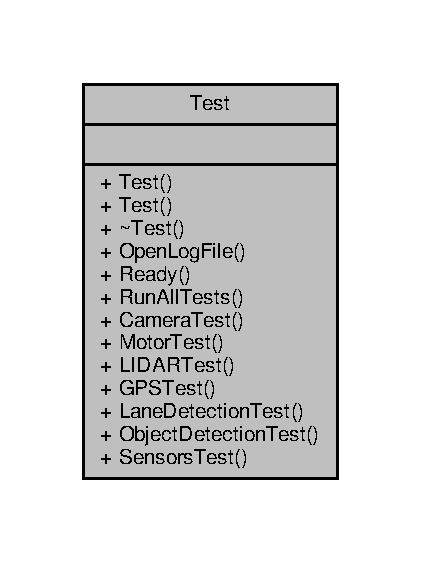
\includegraphics[width=202pt]{d2/da7/classTest__coll__graph}
\end{center}
\end{figure}
\subsection*{Public Member Functions}
\begin{DoxyCompactItemize}
\item 
\mbox{\Hypertarget{classTest_adbe72417514d1a539c5bc6c8babef29b}\label{classTest_adbe72417514d1a539c5bc6c8babef29b}} 
{\bfseries Test} (const char $\ast$logfile)
\item 
\mbox{\Hypertarget{classTest_a25598d6dc97057505907cf4c488cbb5e}\label{classTest_a25598d6dc97057505907cf4c488cbb5e}} 
bool {\bfseries Open\+Log\+File} (const char $\ast$logfile)
\item 
\mbox{\Hypertarget{classTest_a867b28580579e38b0506e564a3b7d337}\label{classTest_a867b28580579e38b0506e564a3b7d337}} 
bool {\bfseries Ready} ()
\item 
\mbox{\Hypertarget{classTest_a3b5613b55d133595ac21a4760cc2a858}\label{classTest_a3b5613b55d133595ac21a4760cc2a858}} 
bool {\bfseries Run\+All\+Tests} ()
\item 
\mbox{\Hypertarget{classTest_a49c03674efed3ff327fbfc4e73d08b79}\label{classTest_a49c03674efed3ff327fbfc4e73d08b79}} 
bool {\bfseries Camera\+Test} ()
\item 
\mbox{\Hypertarget{classTest_a77b8ffb69e4073d0fd8eaf95722ff97e}\label{classTest_a77b8ffb69e4073d0fd8eaf95722ff97e}} 
bool {\bfseries Motor\+Test} ()
\item 
\mbox{\Hypertarget{classTest_afc4a9c7189a8ccd36ad4d3ae6630ef3e}\label{classTest_afc4a9c7189a8ccd36ad4d3ae6630ef3e}} 
bool {\bfseries L\+I\+D\+A\+R\+Test} ()
\item 
\mbox{\Hypertarget{classTest_a3e358c24e43706caba09b9fe6c113621}\label{classTest_a3e358c24e43706caba09b9fe6c113621}} 
bool {\bfseries G\+P\+S\+Test} ()
\item 
\mbox{\Hypertarget{classTest_a0fb05792f614566d0e16da82d926f479}\label{classTest_a0fb05792f614566d0e16da82d926f479}} 
bool {\bfseries Lane\+Detection\+Test} (string filename)
\item 
\mbox{\Hypertarget{classTest_a50f8e04aabd2266d3ee9c86900e85b91}\label{classTest_a50f8e04aabd2266d3ee9c86900e85b91}} 
bool {\bfseries Object\+Detection\+Test} ()
\item 
\mbox{\Hypertarget{classTest_acb268b7a37c9cce085d0659f4747fd4a}\label{classTest_acb268b7a37c9cce085d0659f4747fd4a}} 
bool {\bfseries Sensors\+Test} ()
\end{DoxyCompactItemize}


The documentation for this class was generated from the following files\+:\begin{DoxyCompactItemize}
\item 
/home/soobin/\+Documents/\+Sandbox/\+I\+G\+V/test/test.\+hpp\item 
/home/soobin/\+Documents/\+Sandbox/\+I\+G\+V/test/test.\+cpp\end{DoxyCompactItemize}

%--- End generated contents ---

% Index
\backmatter
\newpage
\phantomsection
\clearemptydoublepage
\addcontentsline{toc}{chapter}{Index}
\printindex

\end{document}
